
\begin{frame}
  \frametitle{Motivation}
  \framesubtitle{ZENO/Walk-on-Spheres}

  \begin{itemize}
    \item ZENO/Walk-on-Spheres is an accelerated implementation of the ZENO computation which is a Monte Carlo
      numerical path integration that yields material properties such as:
    \begin{itemize}
      \item electrostatic capacity
      \item polarizability tensor
      \item intrinsic conductivity 
      \item hydrodynamic radius
      \item translational diffusion constant
      \item and more
    \end{itemize}
  \end{itemize}

\end{frame}

\begin{frame}
  \frametitle{Motivation}
  \framesubtitle{ZENO/Walk-on-Spheres}

  \begin{figure}
    \centering
    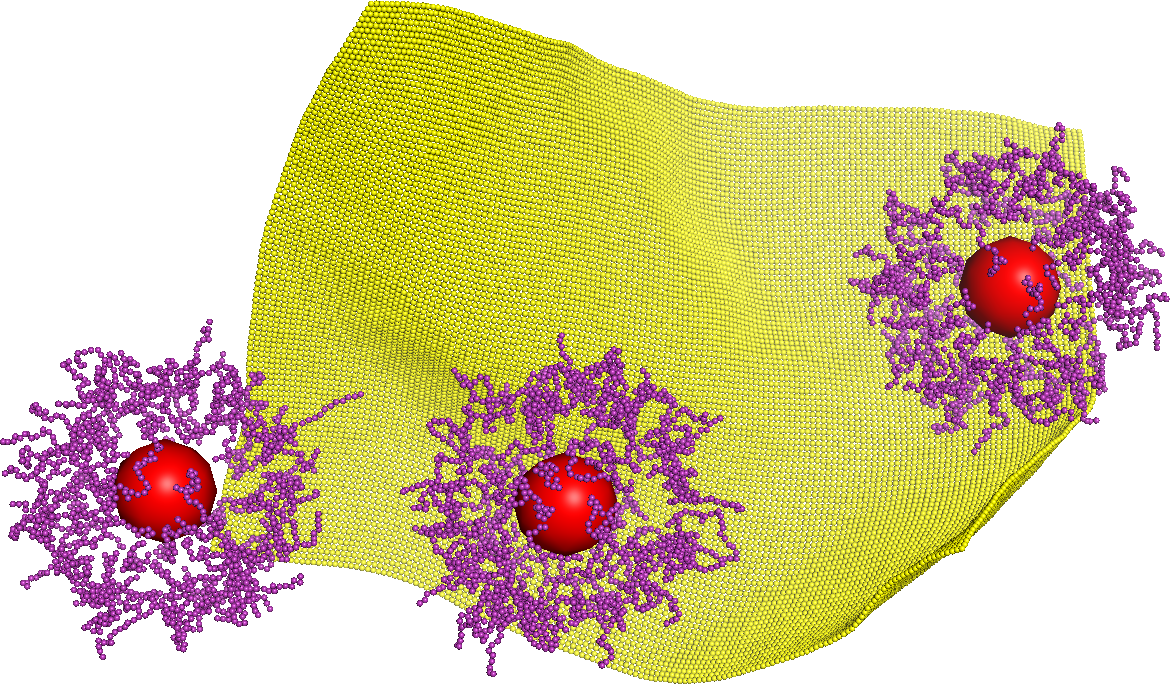
\includegraphics[width=0.7\textwidth]{80000_NOBGCROP.png}
    \caption{DNA-grafted gold nano-particles interacting with a 
    two-dimensional DNA-based origami construct (23115 speheres).}
    \label{fig:80000}
  \end{figure}
\end{frame}

\begin{frame}
  \frametitle{Motivation}
  \framesubtitle{ZENO/Walk-on-Spheres}

  \begin{columns}[T]
    \begin{column}{.5\textwidth}
      \begin{block}{}%
        {\color{white} Walk-on-Spheres accelerates Brownian Motion by jumping %
          to a uniformly distributed point on the surface of a surrounding sphere}
      \end{block}
    \end{column}
    \begin{column}{.5\textwidth}
      \begin{block}{}
        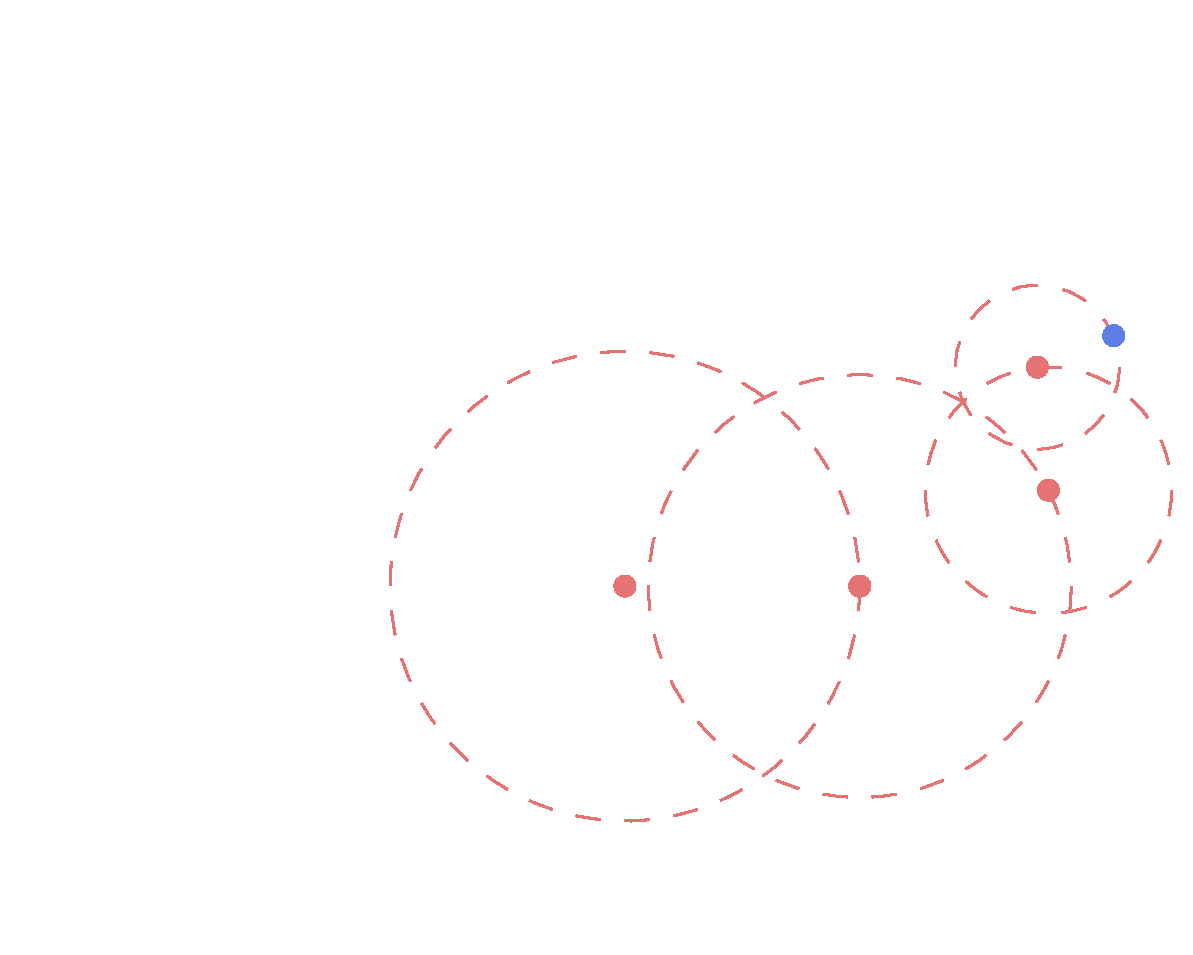
\includegraphics[width=\textwidth]{WoS.pdf}
      \end{block}
    \end{column}
  \end{columns}
\end{frame}

\begin{frame}
  \frametitle{Specification}

  {\usebeamerfont{title}\color{white}
  Improve performance of nearest neighbor search on \kd trees by more compactly organizing tree components
  to reduce cache misses and load instructions.}

\end{frame}
